
\section{Introduction}
\label{sec:Introduction}
%%%%%%%%%%%%%%%%%%%%% Vision %%%%%%%%%%%%%%%%%%%%%%%%%
The goal of this work is to provide and compare multiple actuator morphologies and multiple fabrication processes for realizing soft autonomous fluidic elastomer robots.
%
We experimentally validate these morphologies and processes in the context of extremely soft and highly compliant locomotory robots and manipulators shown in Figure~\ref{fig:intro_new}.
\begin{figure}[!t]
  \centering
  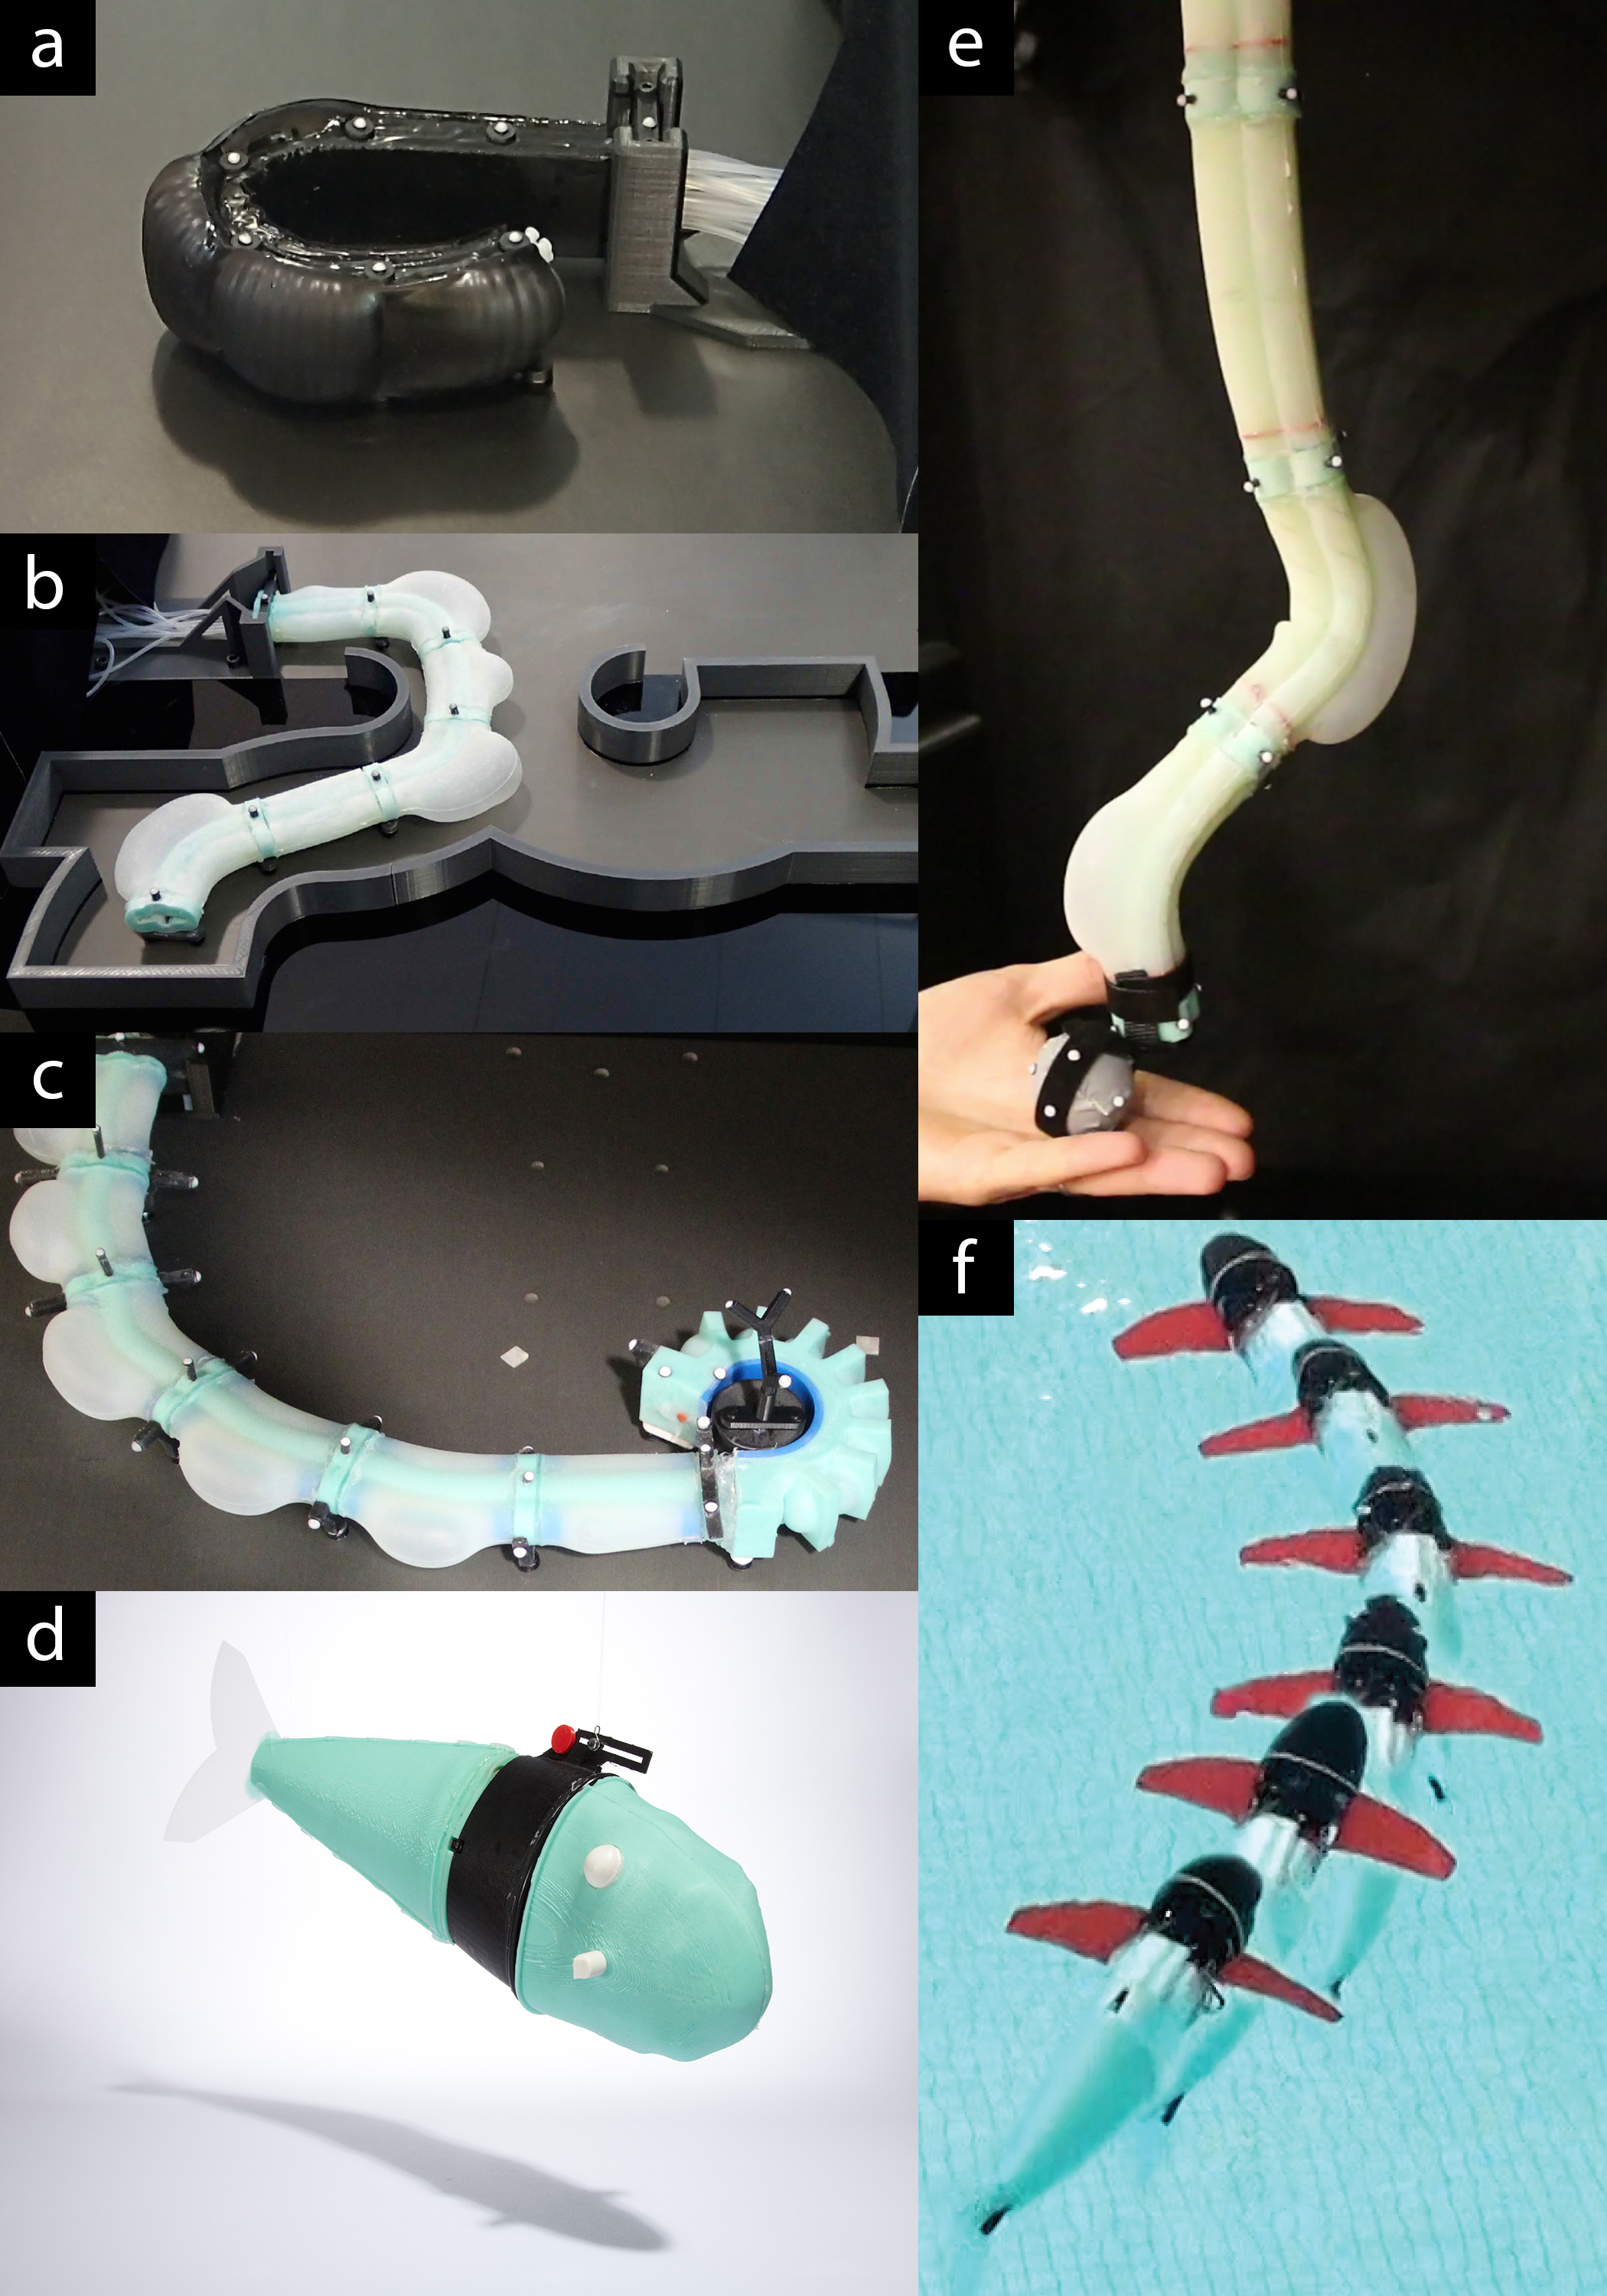
\includegraphics[width=3in]{figures/introduction/intronew.jpg}
  \caption{Extremely soft and highly compliant fluidic elastomer robots. (\textbf{a}) Ribbed planar manipulator \citep{marchese2014design}, (\textbf{b}) Cylindrical planar manipulator \citep{marchese2014whole}, (\textbf{c}) Cylindrical manipulator with gripper \citep{katzschmann2015autonomous}, (\textbf{d}) Self-contained pneumatic fish \citep{marchese2014autonomous}(photo courtesy of Devon Jarvis for popular mechanics), (\textbf{e}) Spatial cylindrical manipulator \citep{marchese2015design}, and (\textbf{f}) Self-contained hydraulic fish \citep{katzschmann2014hydraulic}. }\label{fig:intro_new}
\end{figure}

Soft robots exhibit continuum body motion, large scale deformation, and relatively high compliance compared to traditional rigid-bodied robots \citep{trivedi2008soft}.
%
Such characteristics give this class of robots advantages like the ability to mitigate uncertainty with passive compliance \citep{mcmahan2006field}, perform highly dexterous tasks \citep{deimel2014novel}, and exhibit resiliency \citep{tolley2014resilient}.
%
This work provides a recipe for designing and fabricating soft fluidic elastomer actuators and robotic systems.

%%%%%%%%%%%%%%%%%%%%% Challenges %%%%%%%%%%%%%%%%%%%%%%%%%
\subsection{Challenges}
Recent reviews \citep{trivedi2008soft, trimmer2014journal, lipson2014challenges, majidi2014soft} articulate the challenges associated with creating robots from soft, nonlinear materials.
%
To summarize, current engineering tools are well-suited for rigid-bodied robots and when soft, nonlinear elastic materials are introduced, many of the underlying assumptions of these tools are broken.
%
To create fluidic elastomer robots, we must overcome many technical challenges, many of which have to do with design and fabrication.
%
More specifically, this work addresses the following challenges:
(i) We do not have multi-segment fluidic elastomer locomotory robot nor manipulator designs suitable for automated tasks.
That is, we need to identify appropriate actuator morphologies and ways of assembling these actuators into multi-body robots.
(ii) Consistently reproducing certain properties of soft robots, for example their elasticity or internal channel geometry, is difficult using conventional fabrication techniques.
Accordingly, we must develop fabrication techniques that balance the competing goals of scalability and repeatability with the need for complicated features and shape profiles.

%%%%%%%%%%%%%%%%%%%%% Approach %%%%%%%%%%%%%%%%%%%%%%%%%
\subsection{Approach}
%In this work, we demonstrate that autonomous manipulation with soft fluidic elastomer robots is possible.
First, we review relevant soft actuation technology, design tools, and fabrication processes in Section~\ref{sec:Related Work}.
%
Next, we present the design and characterization of three fluidic elastomer actuator morphologies in Section~\ref{sec:Actuators}.
%
These actuator morphologies are differentiated by their internal channel structure, namely: ribbed, cylindrical, and pleated.
%
Next, we provide three alternative fabrication approaches for reliably fabricating soft actuators and multi-segment robots in Section~\ref{sec:Fabrication}.
%
These processes are lamination-based embedded casting, retractable-pin-based casting, and lost-wax-based casting.
%
Then, we briefly discuss alternative approaches to powering these robots in Section~\ref{sec:Power}.
%
And lastly, we demonstrate how the various actuator morphologies and fabrication processes have been used to realize a variety of soft autonomous systems: locomotory fish-like robots in Section~\ref{sec:Locomotion} and robotic manipulation systems in Section~\ref{sec:Manipulators}.

%%%%%%%%%%%%%%%%%%%%% Contributions %%%%%%%%%%%%%%%%%%%%%%%%%
\subsection{Contributions}
%The primary contribution of this work is a novel power and computational control and planning system for 2D fluidic elastomer manipulation that enable grasp-and-place and planned continuous motion in environments with obstacles.
%This work is first to show that planar manipulation with soft fluidic elastomer robots is possible and first to provide an approach for closed-loop control and planning of such manipulators.
Specifically this work makes the following contributions:
\begin{enumerate}
  \item Three viable fluidic elastomer actuator (FEA) morphologies. That is, a FEA with a (i) ribbed channel structure and embedded transmission lines, (ii) cylindrical channel structure and hollow interior, (iii) seamless pleated channel structure;
  \item Three fabrication processes for reliably manufacturing these FEAs. These are (i) a lamination-based casting process with heterogeneous embedded components, (ii) a retractable-pin-based casting process, (iii) a lost-wax-based casting process;
  \item A survey of recent robots built using these design and fabrication approaches (See Fig.~\ref{fig:intro_new}).
\end{enumerate}
This work significantly extends three previous conference publications: \citep{marchese2014design}, \citep{marchese2014whole}, and \citep{katzschmann2015autonomous} (in revision). %TODO remove if not in revision anymore 